\documentclass[letterpaper,11pt]{article}

\usepackage{graphicx}
\usepackage{multicol}
\usepackage{fullpage}
\usepackage{csquotes}
\usepackage[margin=0.75in,letterpaper]{geometry}
\setlength{\footskip}{15pt}
\setlength{\belowcaptionskip}{9pt}
\usepackage{censor}
\usepackage{floatflt}
\usepackage{xspace}
\usepackage[margin=1cm,skip=9pt]{caption}
\usepackage{ulem}
\usepackage{tikz}
\usepackage{siunitx}
\usetikzlibrary{shadows}

% https://tex.stackexchange.com/questions/5226/keyboard-font-for-latex
\newcommand*\keys[1]{%
  \tikz[baseline=(key.base)]
    \node[%
      draw,
      fill=white,
      drop shadow={shadow xshift=0.25ex,shadow yshift=-0.25ex,fill=black,opacity=0.75},
      rectangle,
      rounded corners=2pt,
      inner sep=1pt,
      line width=0.5pt,
      minimum width=1.1em,
      font=\scriptsize\sffamily
    ](key) {#1\strut}
  ;
}

\linespread{0.95}
\def\degC{$^{\circ}$C }
\def\degf{$^{\circ}$F }
\def\vol #1 {{\bf #1}, $\;\;$}
\def\refer{\par\noindent\hangindent\parindent\hangafter1}


\title{\vspace{-2.0cm}Herzmann Family Christmas Letter 2024}
\author{Daryl Herzmann${}^1$, Elizabeth Herzmann${}^2$, Margaret 
Herzmann${}^3$,\\
Robert Herzmann${}^3$, AND Charlotte Herzmann${}^3$ \\
\textit{${}^1$Corresponding Author},
\it{${}^2$Does all the work},
\it{${}^3$Coincident Children}}
\date{17 December 2024}

\makeatletter
\newenvironment{tablehere}
  {\def\@captype{table}}
  {}

\newenvironment{figurehere}
  {\def\@captype{figure}}
  {}
\makeatother

\newcommand{\Line}[0]{%
  \rule{0cm}{0cm}\\\hrule\rule{0cm}{0cm}%
}

%\addtolength{\textheight}{1.5in}

\begin{document}
\maketitle
\vspace{-0.75cm}
\begin{abstract}
Get excited! It is time again for the annual \textit{quasi}-objective assessment of the Herzmann
family progress and tribulations. Overall, things are pretty, pretty, ...
pretty good (David 2024).
\end{abstract}

\vspace{-0.5cm}

\noindent\makebox[\linewidth]{\rule{\textwidth}{1pt}}

\begin{multicols}{2}

\section{Materials and Methods} 

Our family still comprises Daryl
\enquote{Daryl} (46), Elizabeth \enquote{Liz} (number evenly divisible by 10),
Margaret \enquote{Maggie Moo} (11), Robert \enquote{Rooobert} (10), and
Charlotte \enquote{Friend} (7).

\subsection{Housing and Domestics}

This year featured the addition of four woodland creatures, such that our
house now resembles something from Marty Stouffer's \textit{Wild America}. The
girls have two domestic guinea pigs (\textit{Cavia porcellus}) named 
\enquote{Pebbles} and \enquote{Tessa}. The boy
has two biting gerbils (\textit{Meriones unguiculatus}) named
\enquote{Hermione} and \enquote{Sirius}.  The pigs have
figured out how to politely ask for lettuce via incessant
squeaking. Mom does a disproportionate amount of the feeding and cleaning of the
cages.


\bigskip

\subsection{Conveyances}

Daryl's \textit{Honda Pilot} has fallen in love with frequent visits to the
mechanic for transmission issues.  Its life of tree stump pulling and hauling
fattened cattle to market has taken a toll.  Liz's minivan continues to
clunk along and just crossed 100,000 miles (\SI{161000000}{\meter}). We continue
to boggle which pile of junk will be first gifted to Maggie.

\bigskip

\subsection{The Begetters}

The life-long commitment of marriage seems apace.  Our ${15}^{th}$ wedding anniversary
is expected this coming July and we are planning a trip somewhere nicer than
\textit{Culver's}, perhaps \textit{Arby's}.

Daryl was hoping to use this section to bemoan the magnitude of car driving to
facilitate all the children's activities below, but after preparing the data
to support this hyperbole, Figure 1 tells a different story with daily mileage
still below pre-\textsc{COVID19} levels.  Continued hopes
of marathon running and general fitness remain fleeting.  Work has become
rather interesting as ludomaniacs have discovered wagering on airport
weather station reports and his website is an excellent source of data.

\bigskip

\begin{figurehere}
    \centering   
    \resizebox{.95\columnwidth}{!}{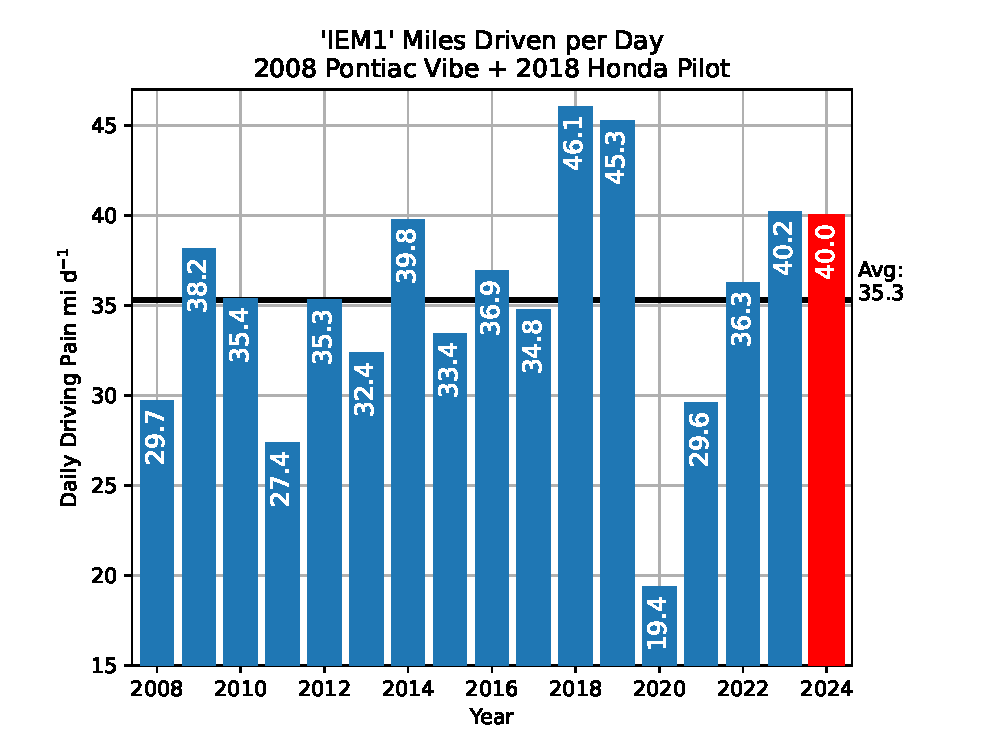
\includegraphics[angle=0]{plots/f1_2024.eps}}
    \caption{Average miles driven per day.}
\end{figurehere}

Liz again opines that nothing is new with her and she continues the
indoctrination of youth at Southview Middle School here in Ankeny.
She is excited to get a
student teacher this spring and all the \sout{tedium}
educational experiences to offload on them.

\section{Miss Charlotte}

Charlotte is in ${2}^{nd}$ grade and loves science time.  She loves dada and
momma as well. She went to her first soccer tournament in Kansas City this year and
loved it so much. She started basketball and what she lacks in stature she
makes up for in enthusiasm, says the coach. Our vacation trip to Chicago was great fun for her
and she enjoyed doing a cartwheel from the Willis Tower Skydeck (Figure 2). She
has her first communion this spring.

\begin{figurehere}
    \centering   
    \resizebox{.95\columnwidth}{!}{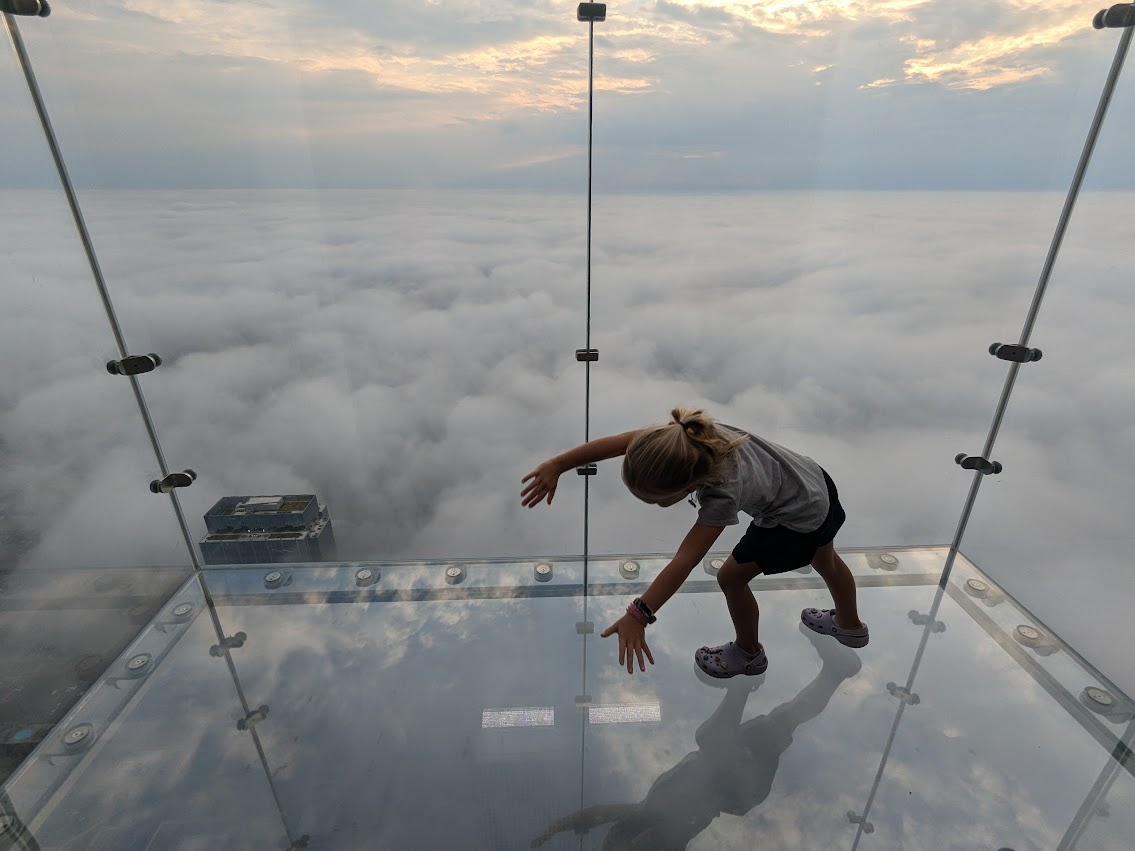
\includegraphics[angle=0]{plots/f2_2024.eps}}
    \caption{Charlotte tempting fate by testing strength of glass at \SI{412}{\meter} AGL.}
\end{figurehere}


\section{Mr Robert}

${5}^{th}$ grader Robert remains a contrarian's contrarian. He loves
to read, unleashes his inner \textit{Beethoven} on the piano, and is now playing somewhat
organized basketball. He started band this year and is playing percussion,
but thankfully it only involves the xylophone and not the drum set. He is on the
yearbook club to limit the number of photos of him in the yearbook. He
enjoys volunteering with his grandfather at the food pantry. He still enjoys
playing computer games when he is not supposed to.

\section{Miss Maggie}

\begin{figurehere}
    \centering   
    \resizebox{.95\columnwidth}{!}{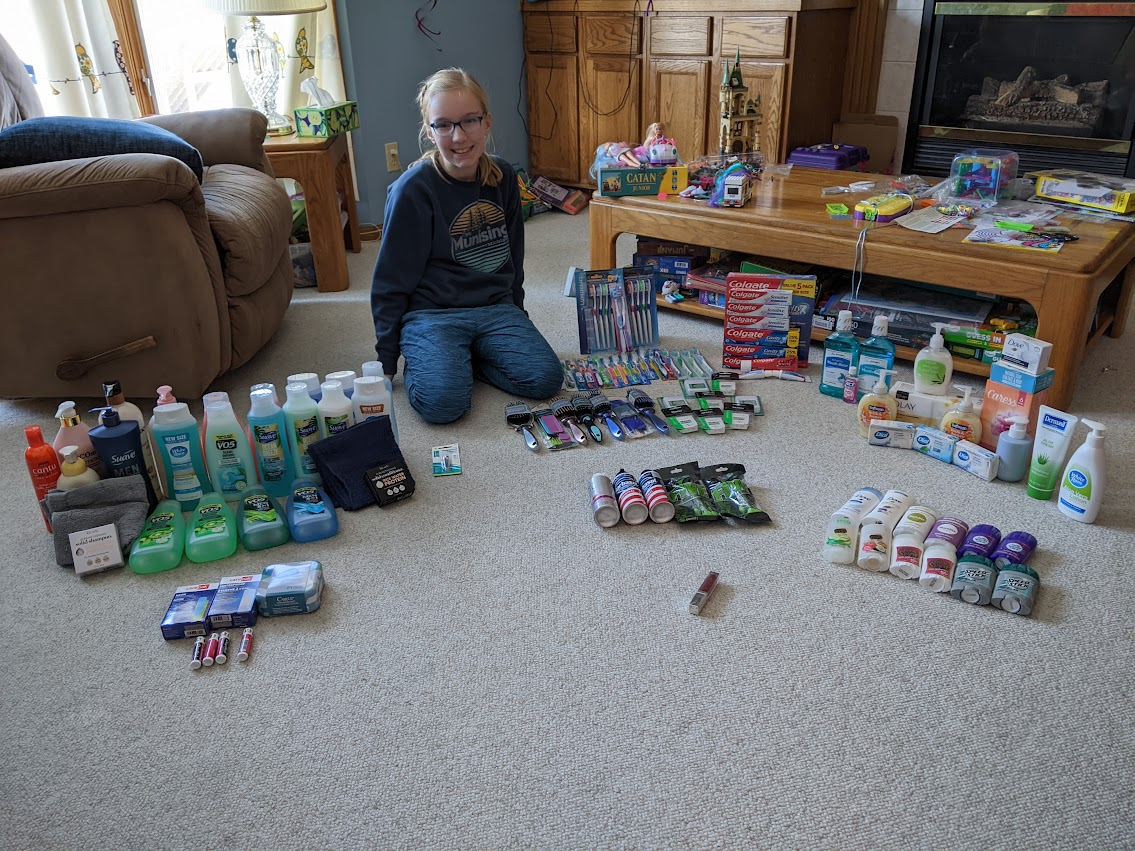
\includegraphics[angle=0]{plots/f3_2024.eps}}
    \caption{Maggie with her 2024 birthday donation haul and associated product placement
    hoping for future sponsorship.}
\end{figurehere}

Maggie is in her first year of middle school as a 6th grader. She is loving all
of her new teachers and has her favorite classes of math and science first thing
in the morning.
She is working hard in all of her classes and is doing great. She is playing
volleyball again this year
and is joining a national team (the highest level) at Ankeny Volleyball Academy (AVBA).
She continues 
to do dance and is now starting to learn dances for her spring recital.
She is also in band and just 
performed in her first concert. This year she got the opportunity to do choir
and enjoys it.
She continues to show her creativity by making the family Christmas card this year.
She is also showing her leadership skills and is a great role model for her
younger siblings (\textit{editorial: her words, not mine}).
She is once again giving up her birthday presents to get toiletry items for
the food pantry.


\section{Family Trips}

We made two family trips over the summer break.  First was an urban
adventure to Chicago during the hottest week of the year.
We stayed at a hotel downtown and were able to walk
to the standard tourist attractions.  Maggie was thrilled to see Lake Michigan
native dolphins for the first time at \textit{Shedd Aquarium}. Charlotte was
impressed by the buildings slightly taller than those in Ankeny. Daryl was
impressed by the amount of noise the 3 AM street racers make. 
We also visited Wrigley Field and caught
a winning Cubs game whilst there.

The second, albeit shorter, trip was to Kansas City for the hottest days of
its year as well. The Chicago Cubs were conveniently
playing there as well.  The Cubs won again, so we plan on
attending all Cubs games next year to ensure a \textbf{162-0} record.

\bigskip

\emph{Acknowledgments} Our family wishes to thank you for the generous 
support, prayers, cards, gifts, and visits you have provided us in the past
year. Color page charges continue to be the bane of my existence.
Satiating Reviewer Number 2 needlessly delayed publication. Full
\LaTeX\xspace source of this letter can be found on Daryl's GitHub page. 

\section{References}

\refer David, Larry. Personal communication, 30 Feb 2024.
\refer GitHub. \texttt{https://github.com/akrherz/akrherz}, last viewed on 7 Dec 2024.

\end{multicols}

\end{document}
